\chapter{Проектирование подсистемы популяций и суточных сценариев}
\label{chap:population}

\section{Архитектура управления популяцией и непрерывность поездок}
\label{sec:population_arch}

Для обеспечения физической реалистичности динамического моделирования разработан программный интерфейс \texttt{IPopulationManager}. В отличие от упрощенных симуляторов, в которых каждая поездка генерируется независимым случайным спавном с последующим удалением автомобиля, в разработанном модуле реализована концепция сохранения идентичности агентов и непрерывных цепочек перемещений (\emph{trip chaining}, \emph{zero-teleportation}).

Каждому агенту при инициализации назначается базовая точка проживания $e_{\text{home}} \in E$ и точка регулярного притяжения $e_{\text{work}} \in E$. После завершения утренней поездки автомобиль не уничтожается, а переводится в режим ожидания на парковке целевого ребра, сохраняя свое физическое пространственное положение. Вечерняя обратная поездка начинается непосредственно из текущей точки нахождения агента, что исключает телепортации между выездами и обеспечивает баланс входящих и выходящих транспортных потоков в районах города.

\section{Конечный автомат жизненного цикла агента}
\label{sec:agent_fsm}

Поведение каждого транспортного средства в симуляторе формализовано в виде детерминированного конечного автомата, граф состояний которого представлен на рисунке~\ref{fig:agent_lifecycle}.

\begin{figure}[h!]
\centering
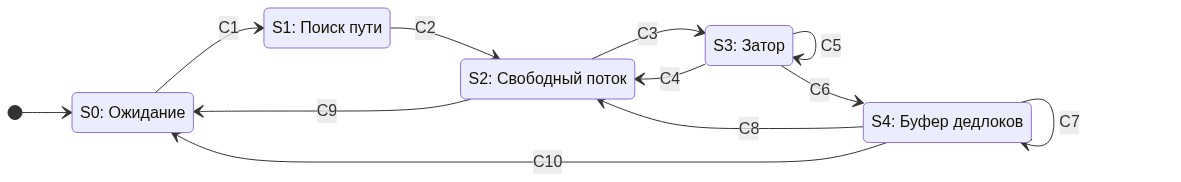
\includegraphics[width=0.85\textwidth]{assets/mermaid/png/01_agent_lifecycle.png}
\caption{Граф состояний конечного автомата жизненного цикла транспортного агента (переходы $C_1 \dots C_{10}$)}
\label{fig:agent_lifecycle}
\end{figure}

На графе автомата элементарные переходы между состояниями обозначены кодами $C_1 \dots C_{10}$:
\begin{itemize}
    \item $C_1$ ($S_0 \to S_1$) --- переход из режима стоянки в режим запроса пути при наступлении времени поездки по суточному графику;
    \item $C_2$ ($S_1 \to S_2$) --- успешное получение пути от сервиса маршрутизации и выезд в свободный поток;
    \item $C_3$ ($S_2 \to S_3$) --- переход в очередь на стоп-линии при исчерпании физической емкости следующего ребра;
    \item $C_4$ ($S_3 \to S_2$) --- освобождение следующего ребра ниже порога $70\%$ и сброс таймера затора;
    \item $C_5$ ($S_3 \to S_3$) --- переход на короткое ребро при сохранении затора с продолжением отсчета простоя (\texttt{conttimer});
    \item $C_6$ ($S_3 \to S_4$) --- превышение порогового интервала ожидания ($t_{\text{wait}} \ge 130$~с) и эвакуация в буфер;
    \item $C_7$ ($S_4 \to S_4$) --- виртуальное продвижение со скоростью BPR в обход физического кольца затора;
    \item $C_8$ ($S_4 \to S_2$) --- возврат из виртуального буфера на сеть при падении загрузки ребра ниже $70\%$;
    \item $C_9, C_{10}$ ($S_2 \to S_0, S_4 \to S_0$) --- прибытие в точку назначения и возврат на стоянку.
\end{itemize}

Подробное описание состояний $S_0 \dots S_4$ и формальных условий переходов приведено в таблицах~\ref{tab:agent_states} и~\ref{tab:agent_transitions}.

\begin{table}[h!]
\centering
\caption{Характеристика дискретных состояний агента}
\label{tab:agent_states}
\small
\begin{tabularx}{\textwidth}{|c|l|X|}
\hline
\textbf{Обозн.} & \textbf{Наименование} & \textbf{Физический смысл и назначение состояния} \\ \hline
$S_0$ & \texttt{INACTIVE} & Пассивное состояние. Автомобиль находится на стоянке у дома или работы; поездка не выполняется. \\ \hline
$S_1$ & \texttt{WAITING\_ROUTE} & Ожидание ответа роутера. Агент активирован по суточной квоте, сформирован асинхронный запрос пути. \\ \hline
$S_2$ & \texttt{ACTIVE\_FREE\_FLOW} & Движение в свободном потоке. Агент перемещается по ребру со скоростью $v_{e,\text{free}}$ или BPR. \\ \hline
$S_3$ & \texttt{ACTIVE\_QUEUE} & Стояние в физической очереди ($v = 0$~м/с) на стоп-линии из-за занятости следующего ребра ($load + 1 > jam\_cap$). \\ \hline
$S_4$ & \texttt{VIRTUAL\_BUFFER} & Виртуальный буфер заторов. Снятие с дороги при $t_{\text{wait}} \ge T_{\text{teleport}}$ с разрывом кольца дедлока. \\ \hline
\end{tabularx}
\end{table}

\begin{table}[h!]
\centering
\caption{События и условия переходов конечного автомата агента}
\label{tab:agent_transitions}
\small
\begin{tabularx}{\textwidth}{|c|c|X|}
\hline
\textbf{Код} & \textbf{Переход} & \textbf{Условие активации и физическое событие} \\ \hline
$C_1$ & $S_0 \to S_1$ & Наступление времени выезда по суточному профилю ($N_{\text{active}} < N_{\text{target}}$). \\ \hline
$C_2$ & $S_1 \to S_2$ & Успешное получение кратчайшего маршрута от сервиса роутинга. \\ \hline
$C_3$ & $S_2 \to S_3$ & Достижение стоп-линии при исчерпании емкости следующего ребра ($V_{e_{\text{next}}} + 1 > C_{e_{\text{next}},\text{jam}}$). \\ \hline
$C_4$ & $S_3 \to S_2$ & Освобождение следующего ребра ниже порога $J_{\text{thresh}} = 70\%$; сброс таймера затора в 0. \\ \hline
$C_5$ & $S_3 \to S_3$ & Переход на короткое ребро при сохранении затора ($\ge 70\%$); инвариант \texttt{conttimer}. \\ \hline
$C_6$ & $S_3 \to S_4$ & Превышение порогового интервала ожидания ($t_{\text{wait}} \ge T_{\text{teleport}} = 130$~с). \\ \hline
$C_7$ & $S_4 \to S_4$ & Виртуальное продвижение со скоростью $v_{\text{virt}}$ по забитым сегментам. \\ \hline
$C_8$ & $S_4 \to S_2$ & Выход из виртуального буфера: физическое ребро освободилось ($V_e / C_{e,\text{jam}} \le 70\%$). \\ \hline
$C_9$ & $S_2 \to S_0$ & Завершение маршрута; прибытие в целевую точку назначения. \\ \hline
$C_{10}$ & $S_4 \to S_0$ & Завершение маршрута в буферном слое (финишная точка достигнута). \\ \hline
\end{tabularx}
\end{table}

\section{Моделирование суточных циклов активности и дефицитный спавн}
\label{sec:diurnal_control}

Интенсивность дорожного движения в течение суток задается суточным объемным профилем активности $R(t) \in [0.125, 1.0]$. Параметры суточного профиля активности приведены в таблице~\ref{tab:diurnal_profile}.

\begin{table}[h!]
\centering
\caption{Параметры суточного профиля активной доли автопарка}
\label{tab:diurnal_profile}
\begin{tabularx}{\textwidth}{|c|c|X|}
\hline
\textbf{Интервал времени (ч)} & \textbf{Доля активных $R(t)$} & \textbf{Характеристика транспортного потока} \\ \hline
00:00 -- 06:00 & $0.125$ ($12.5\%$) & Ночной минимум активности сети \\ \hline
06:00 -- 09:00 & $0.500$ ($50.0\%$) & Утреннее нарастание трудовых корреспонденций \\ \hline
09:00 -- 12:00 & $0.875$ ($87.5\%$) & Утренний час пик \\ \hline
12:00 -- 15:00 & $0.500$ ($50.0\%$) & Дневной межпиковый спад \\ \hline
15:00 -- 18:00 & $0.750$ ($75.0\%$) & Предвечернее нарастание нагрузки \\ \hline
18:00 -- 21:00 & $1.000$ ($100.0\%$) & Основной вечерний час пик (максимум) \\ \hline
21:00 -- 00:00 & $0.250$ ($25.0\%$) & Вечерний спад и возвращение на стоянки \\ \hline
\end{tabularx}
\end{table}

Для общего автопарка $N_{\max} = 70\,000$ автомобилей целевое количество агентов на дорогах в момент времени $t$ составляет:
\begin{equation}
N_{\text{target}}(t) = N_{\max} \cdot R(t).
\label{eq:target_agents}
\end{equation}

Фактическое число автомобилей, одновременно находящихся в движении в момент времени $t$, вычисляется суммированием всех активных категорий:
\begin{equation}
N_{\text{active}}(t) = N_{\text{free}}(t) + N_{\text{queue}}(t) + N_{\text{buffer}}(t) + N_{\text{waiting\_route}}(t).
\label{eq:active_agents_sum}
\end{equation}

Управление популяцией осуществляется по принципу \textbf{дефицитного спавна}:
\begin{enumerate}
    \item В каждый дискретный шаг симуляции проверяется баланс:
    \begin{equation}
    \Delta N(t) = \max\left(0, \; N_{\text{target}}(t) - N_{\text{active}}(t)\right).
    \label{eq:spawn_deficit}
    \end{equation}
    \item Если на дорогах наблюдается дефицит ($\Delta N(t) > 0$), из спящего пула $S_0$ активируется порция агентов размером $\min(\Delta N(t), \text{quota})$, которым назначается маршрут.
    \item Если фактическое число агентов превышает целевой уровень ($N_{\text{active}}(t) \ge N_{\text{target}}(t)$), генерация новых поездок полностью блокируется ($\Delta N = 0$).
\end{enumerate}

Принципиально важно, что в разработанной системе отсутствует механизм принудительного деспавна активных автомобилей при спаде профиля активности. Спад кривой $N_{\text{active}}(t)$ к целевым ночным значениям происходит исключительно за счет естественного завершения поездок и перехода агентов в состояние $S_0$. Таким образом, способность кривой активной популяции повторять профиль $R(t)$ без застревания на верхних уровнях является строгим критерием отсутствия дедлоков в симуляторе.

\section{Пространственная маятниковая миграция на графе Казани}
\label{sec:spatial_migration}

Структура корреспонденций автопарка разделена на четыре группы:
\begin{enumerate}
    \item \textbf{Маятниковый поток} (\emph{Commuters}, 65\%): регулярные утренние поездки из спальных районов в центральную деловую зону и вечерние возвращения в жилые массивы;
    \item \textbf{Коммерческий транспорт} (\emph{Commercial}, 20\%): циклические поездки грузового транспорта и такси со случайным блужданием между коммерческими объектами;
    \item \textbf{Общественный транспорт} (\emph{Public Transport}, 5\%): кольцевые маршруты с фиксированными промежуточными остановками;
    \item \textbf{Фоновый случайный шум} (\emph{Random}, 10\%): произвольные корреспонденции между периферийными узлами.
\end{enumerate}

Координаты опорных узлов притяжения маятниковой миграции приведены в таблице~\ref{tab:spatial_hubs}.

\begin{table}[h!]
\centering
\caption{Опорные пространственные узлы тяготения г.~Казани}
\label{tab:spatial_hubs}
\small
\begin{tabularx}{\textwidth}{|L|c|c|c|L|}
\hline
\textbf{Наименование зоны} & \textbf{Широта} & \textbf{Долгота} & \textbf{Вес} & \textbf{Назначение} \\ \hline
Центральный деловой район & $55.7879$ & $49.1221$ & $0.70$ & Деловая и коммерческая активность \\ \hline
Жилой массив «Квартала» & $55.8285$ & $49.1245$ & $0.40$ & Спальный район (Ново-Савиновский) \\ \hline
Жилой массив «Горки-Азино» & $55.7645$ & $49.2145$ & $0.40$ & Спальный район (Приволжский) \\ \hline
Авиастроительный район & $55.8550$ & $49.0850$ & $0.20$ & Промышленно-жилая зона \\ \hline
Пригородный хаб «Иннополис» & $55.7440$ & $48.7450$ & $0.35$ & Западный пригородный коридор \\ \hline
Пригородный хаб «Высокая Гора» & $55.9120$ & $49.3050$ & $0.35$ & Северо-восточный коридор \\ \hline
Пригородный хаб «Салават Купере» & $55.8340$ & $48.9350$ & $0.30$ & Северо-западный жилой кластер \\ \hline
\end{tabularx}
\end{table}


\section{Алгоритмическая реализация механизма conttimer}
\label{sec:conttimer_algo}

Блок-схема адаптированного алгоритма разрешения дедлоков и непрерывного таймера ожидания представлена на рисунке~\ref{fig:deadlock_conttimer}.

\begin{figure}[h!]
\centering
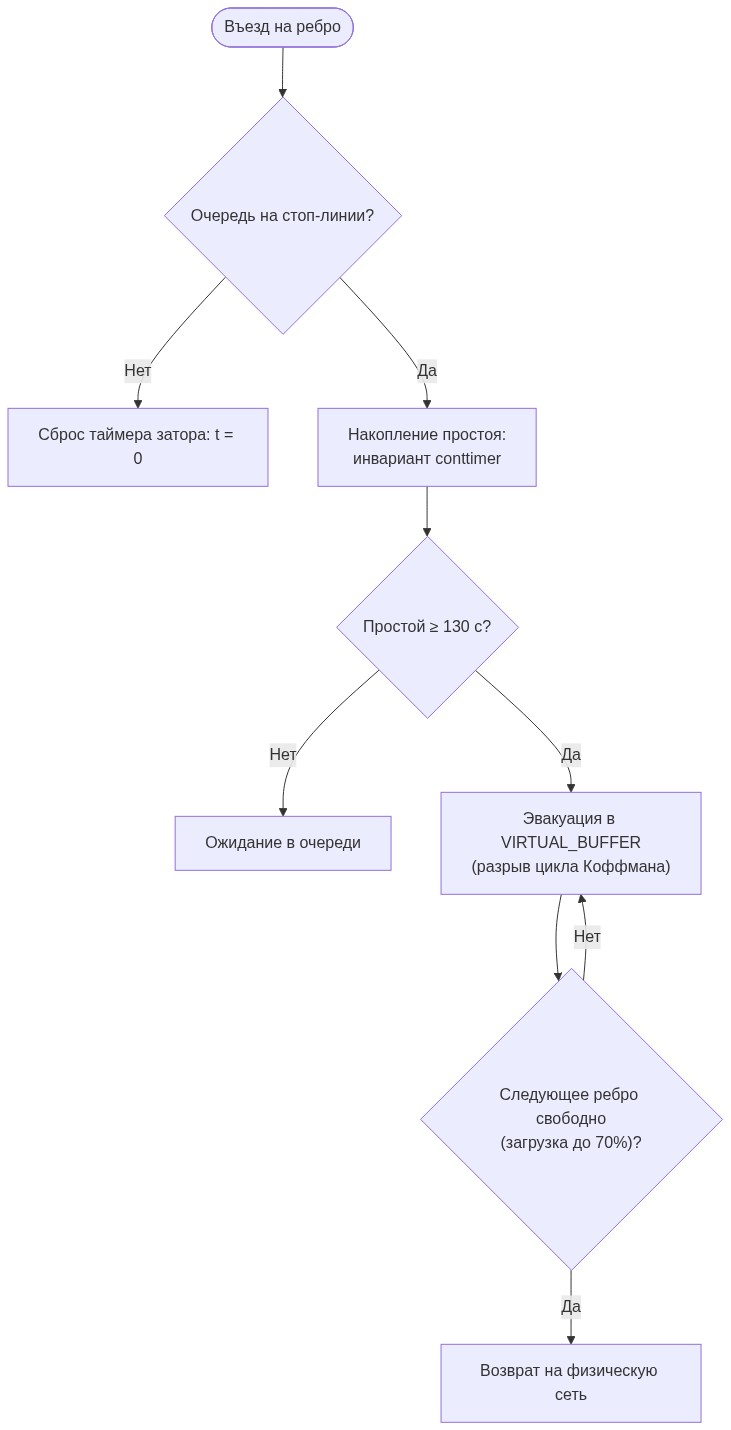
\includegraphics[width=0.6\textwidth]{assets/mermaid/png/02_deadlock_conttimer.png}
\caption{Блок-схема алгоритма разрешения дедлоков и инварианта непрерывного таймера \texttt{conttimer}}
\label{fig:deadlock_conttimer}
\end{figure}

Алгоритм функционирует следующим образом:
\begin{itemize}
    \item При приближении агента к концу ребра проверяется доступность следующего звена маршрута. Если физическая емкость исчерпана ($V_{e_{\text{next}}} + 1 > C_{e_{\text{next}},\text{jam}}$), агент фиксируется на стоп-линии, переводится в состояние $S_3$ (\texttt{ACTIVE\_QUEUE}), и в очередь ожидания заносится отметка времени начала затора $t_{\text{start}}$.
    \item В каждом цикле вычисляется суммарное время ожидания $\Delta t_{\text{wait}} = t_{\text{curr}} - t_{\text{start}}$. Если время превышает порог $T_{\text{teleport}} = 130$~с, агент снимается с физического ребра, декрементируя счетчики $V_e$ и $Q_e$, что разрывает цикл Коффмана. Агент переходит в статус $S_4$ (\texttt{VIRTUAL\_BUFFER}).
    \item В момент перехода автомобиля на следующее ребро проверяется его относительная загрузка. Если ребро свободно ($V_e / C_{e,\text{jam}} < 0.70$), таймер затора сбрасывается ($t_{\text{start}} = 0$). Если же ребро также загружено ($\ge 70\%$), таймер $t_{\text{start}}$ сохраняет свое накопленное значение (\texttt{conttimer}), предотвращая обнуление времени простоя на коротких звеньях сети.
\end{itemize}
